% !TeX program = pdflatex
% !TeX encoding = UTF-8
%=======================================================================
%  GRIS-NOT-001  ·  Plantilla de notas rápidas para la memoria
%  Proyecto 00503 - Generator inspection robotic system · Mecanalisis
%  Identidad: GRIS-IDENTIDAD-001 v1.4
%-----------------------------------------------------------------------
%  CÓMO USARLA (en 3 pasos)
%
%   1. Copiá este archivo con el código de la nota:
%         memoria/notas/02489-00-MC007.tex
%      El número (###) es correlativo: mirá la última nota y sumá uno.
%
%   2. Completá los cuatro datos del bloque «DATOS DE LA NOTA».
%
%   3. Escribí:
%        · Resultados (obligatorio, siempre primero): lo que se sabe
%          ahora que antes no se sabía. Frases cortas, con números.
%        · El resto es libre. Usá los títulos que te sirvan, o ninguno.
%
%   Compilar:  pdflatex 02489-00-MC007.tex
%   En Overleaf: subí el .tex y logo-gris.pdf.
%
%  LOGO: se usa «logo-gris.pdf» (GRIS-LOGO-003, reducido) de esta carpeta
%  o de ../plantilla/. Si falta, se escribe «GRIS» como marcador.
%=======================================================================
\documentclass[11pt,a4paper]{article}

%=======================================================================
%  DATOS DE LA NOTA  ← lo único que hay que tocar arriba
%=======================================================================
\newcommand{\codigo}{02489-00-MC001}          % 02489-00-MC###
\newcommand{\titulo}{Torque admisible de los engranajes cónicos de la rueda}
\newcommand{\autor}{Matías Gaviño}
\newcommand{\fecha}{24/09/2026}                    % o p. ej. {24/09/2026}

%=======================================================================
%  ESTILO  (no hace falta tocar nada de aquí hasta \begin{document})
%=======================================================================
\usepackage[T1]{fontenc}
\usepackage[utf8]{inputenc}
\usepackage[spanish,es-noshorthands,es-tabla]{babel}
\usepackage{lmodern}
\usepackage[a4paper,top=3.0cm,bottom=2.4cm,left=2.4cm,right=2.4cm,
            headheight=20pt,headsep=1.2cm,footskip=1.1cm]{geometry}
\usepackage{microtype}
\usepackage{xcolor}
\usepackage{graphicx}
\usepackage{booktabs}
\usepackage{array}
\usepackage{enumitem}
\usepackage{titlesec}
\usepackage{fancyhdr}
\usepackage{caption}
\usepackage[hidelinks]{hyperref}

% --- colores -----------------------------------------------------------
\definecolor{gris-naranja}{HTML}{FF7A00}   % naranja institucional
\definecolor{tinta}{HTML}{1E2328}
\definecolor{gris-medio}{HTML}{6B7280}
\definecolor{gris-linea}{HTML}{DADDE1}
\color{tinta}

\hypersetup{pdftitle={\codigo\ -- \titulo}, pdfauthor={\autor},
            colorlinks=true, linkcolor=tinta, urlcolor=tinta}

% --- logo ---------------------------------------------------------------
\graphicspath{{./}{../../plantilla/}{figuras/}}
\newcommand{\logogris}{%
  \IfFileExists{logo-gris.pdf}
    {
\includegraphics[height=16pt]{logo-gris.pdf}}
    {\IfFileExists{../../plantilla/logo-gris.pdf}
      {
\includegraphics[height=16pt]{../../plantilla/logo-gris.pdf}}
      {{\fontsize{18}{18}\selectfont\bfseries\sffamily\color{gris-naranja}GRIS}}}}

% --- tipografía del cliente (código documental) --------------------------
% Geogrotesque no es libre; se usa Roboto Condensed Bold, que viene con
% TeX Live y Overleaf y tiene el mismo aire que el logo.
\newcommand{\fuentecliente}{\fontfamily{Roboto-TLF}\fontseries{bc}\selectfont}

% --- encabezado y pie ---------------------------------------------------
\pagestyle{fancy}
\fancyhf{}
\renewcommand{\headrulewidth}{0.4pt}
\renewcommand{\headrule}{\vspace{3pt}{\color{gris-linea}\hrule height \headrulewidth}}
\fancyhead[L]{\logogris}
\fancyhead[R]{{\fuentecliente\fontsize{12}{12}\selectfont\color{gris-medio}\codigo}}
\fancyfoot[R]{\footnotesize\color{gris-medio}\thepage}

% --- títulos numerados ----------------------------------------------------
\setcounter{secnumdepth}{2}
\titleformat{\section}{\large\bfseries}{\thesection}{0.8em}{}
\titleformat{\subsection}{\normalsize\bfseries}{\thesubsection}{0.8em}{}
\titlespacing*{\section}{0pt}{16pt}{5pt}
\titlespacing*{\subsection}{0pt}{11pt}{3pt}

% --- texto ------------------------------------------------------------------
\setlength{\parindent}{0pt}
\setlength{\parskip}{6pt}
\linespread{1.05}
\setlist{topsep=2pt, itemsep=2pt, parsep=0pt, leftmargin=1.2em}
\setlist[itemize]{label={\raisebox{0.15ex}{\small$\bullet$}}}
\captionsetup{font={small,color=gris-medio}, labelfont=bf, skip=5pt}
\renewcommand{\arraystretch}{1.25}

% --- cabecera de la nota ------------------------------------------------------
\newcommand{\cabecera}{%
  \thispagestyle{fancy}%
  {\fontsize{20}{24}\selectfont\bfseries\titulo\par}%
  \vspace{5pt}%
  {\small\color{gris-medio}\fecha\quad·\quad\autor\par}%
  \vspace{6pt}}

% --- ayudas opcionales --------------------------------------------------------
% \figura{archivo}{ancho}{pie}
\newcommand{\figura}[3]{%
  \begin{figure}[htbp]\centering
    \includegraphics[width=#2\linewidth]{#1}\caption{#3}
  \end{figure}}

% --- paquetes adicionales de esta nota --------------------------------------
\usepackage{amsmath}
\usepackage{float}
\usepackage{tabularx}
\usepackage{xspace}
\graphicspath{{figuras/}}
\newcommand{\Nm}{\,N\,m\xspace}

%=======================================================================
\begin{document}
\cabecera

%-----------------------------------------------------------------------
%  RESULTADOS  (siempre primero, lo único obligatorio)
%-----------------------------------------------------------------------
\section{Resultados}
Torque admisible por engranaje del par cónico 1:1 a 90° de la rueda, según Shigley
(cap.~15, método AGMA), con confiabilidad del 95\,\%, torque en ambos sentidos y 10~años de uso.
Todas las mejoras respetan $d_a\le11{,}5$~mm.

\begin{table}[H]\centering\small\setlength{\tabcolsep}{3.6pt}
\begin{tabular}{l r ccc cc r}
\toprule
 & & \multicolumn{3}{c}{Torque normal [N\,m]} & \multicolumn{2}{c}{Pico de 10 s [N\,m]} & \\
\cmidrule(lr){3-5}\cmidrule(lr){6-7}
Diseño & $d_a$ [mm] & 0,5 rpm & 50 rpm & 100 rpm & 0 rpm & 100 rpm & vs.\ actual\\
\midrule
KG M50S20 actual, 170 HB   & 10,71 & 0,152 & 0,098 & \textbf{0,090} & 0,229 & \textbf{0,157} & 1,0\\
KG M50S20 actual, 200 HB   & 10,71 & 0,173 & 0,112 & \textbf{0,108} & 0,261 & \textbf{0,179} & 1,2\\
KG M50B20, latón                  & 10,71 & 0,074 & 0,048 & 0,046 & 0,111 & 0,076 & 0,5\\
m\,0,5 z20, SCM440 300 HB         & 10,71 & 0,243 & 0,157 & \textbf{0,151} & 0,366 & \textbf{0,251} & 1,7\\
m\,0,5 z20, SCM415 carburizada    & 10,71 & 0,481 & 0,310 & \textbf{0,299} & 0,724 & \textbf{0,496} & 3,3\\
m\,0,6 z17, SCM415 carburizada    & 11,05 & 0,557 & 0,358 & \textbf{0,346} & 0,838 & \textbf{0,573} & 3,9\\
\bottomrule
\end{tabular}
\end{table}

\begin{itemize}
  \item \textbf{Mitra actual KG M50S20:} admite entre \textbf{0,090 y 0,108\Nm} en servicio continuo a 100~rpm, según la dureza
        real del S45C (170~HB cota baja, 200~HB típico; KG no la especifica). En picos admite 0,157 a 0,179\Nm. \textbf{Hay que medir la dureza.}
  \item \textbf{Coincide con el datasheet de KG.} KG publica 0,143\Nm a 100~rpm para carga en un sentido; con su propia regla
        para carga en ambos sentidos (2/3) da \textbf{0,095\Nm}, dentro del rango anterior. La diferencia aparente venía de
        supuestos conservadores de la versión anterior de esta nota (sec.~\ref{sec:datasheet}).
  \item \textbf{KG no publica el picado.} Con 170~HB el picado es el límite a 100~rpm; con 200~HB pasa a mandar la flexión.
  \item \textbf{No hay mejora de stock dentro de 11,5~mm:} la siguiente mitra KG (M50S25) mide 13,2~mm.
  \item \textbf{Mejora sin cambiar la geometría:} la misma mitra m\,0,5 z20 a medida en SCM440 bonificado (×1,7)
        o en SCM415 carburizado (×3,3). Entra en el mismo lugar que la actual.
  \item \textbf{Máximo dentro de 11,5~mm:} m\,0,6 z17 carburizada (×3,9; 0,346\Nm continuo), pero cambia la distancia de montaje.
  \item \textbf{Para decidir, vida con incertidumbre} (sec.~\ref{sec:mc}; dureza medida $\approx$240~HB, ida y vuelta frecuente, más de
        20 picos por hora): probabilidad de llegar a \textbf{2~años (576~h)} con el uso real: KG sin tratar \textbf{50\,\%},
        KG nitrocarburada \textbf{79\,\%}, carburizadas \textbf{100\,\%}. Con el motor a pleno: m\,0,6 z18 carburizada
        \textbf{96\,\%}, m\,0,5 z20 carburizada 87\,\%, KG $\le$1\,\%. Con picos frecuentes manda la fatiga a flexión.
  \item \textbf{Vida en horas con un único criterio} (sec.~\ref{sec:vida}, 100~rpm, 24~h por mes): con el uso real medido
        (0,05--0,20\Nm, picos de 0,30) la KG sin tratar dura $\approx$250~h con 200~HB y no es admisible con 170~HB; nitrocarburada,
        \textbf{$\approx$1100~h (170~HB) a $\approx$7400~h (200~HB)}, al límite (margen $\approx$1). Con el motor a pleno
        (0,40\Nm, picos de 0,50) ninguna mitra KG sirve.
  \item \textbf{Óptimo con $d_a\le12$~mm: m\,0,6 z18 carburizada} ($d_a=11{,}65$~mm): no limita ni con el motor a pleno
        (margen 1,33 continuo, 1,84 picos). Reemplazo directo: m\,0,5 z20 carburizada con la geometría de KG (margen 1,16).
  \item \textbf{Flexión del S45C con 24~h por mes} (sec.~\ref{sec:flexion}): a 100~rpm admite \textbf{0,094 a 0,113\Nm} en continuo
        con los factores de la nota y 10 a 2~años de vida; con factores optimistas sin cambiar el montaje, \textbf{0,144 a 0,172\Nm}.
        Acortar la vida suma solo un 5\,\%. El diente se rompe de un golpe recién a $\approx$1,2--1,4\Nm.
  \item Los dos prisioneros M2,5 admiten 0,28\Nm: alcanzan para la mitra actual, no para las mejoras. Estas necesitan
        arrastre positivo (plano en D o pasador) y, las carburizadas, eje de 4~mm. Todo vale solo con \textbf{grasa EP}.
\end{itemize}

\begin{figure}[H]\centering
  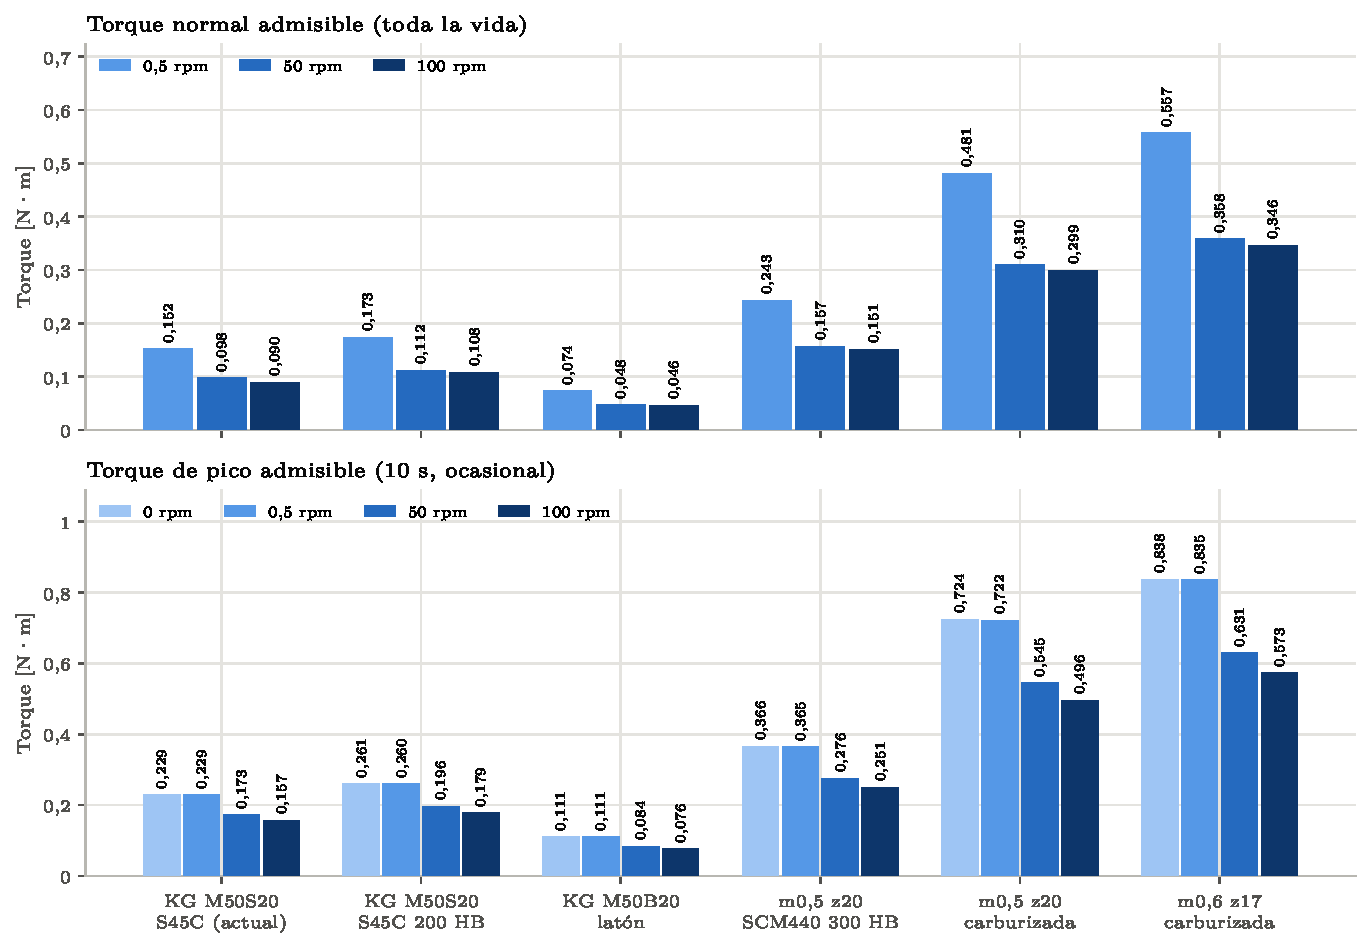
\includegraphics[width=\linewidth]{fig_resumen.pdf}
  \caption{Torque admisible de cada diseño en servicio normal y en picos de 10~s.}
  \label{fig:resumen}
\end{figure}

%-----------------------------------------------------------------------
\section{Datos y supuestos}
El par transmite el giro de un motor BLDC a la rueda de un carro, con ejes a 90° y relación 1:1.

\begin{table}[H]\centering\small
\begin{tabularx}{\linewidth}{l X l}
\toprule
Dato & Valor & Origen\\\midrule
Par & Cónicos rectos iguales (mitras), 1:1, $\Sigma=90^\circ$ & pedido\\
Envolvente & $d_a\le11{,}5$~mm para las mejoras (la actual mide 10,71~mm) & pedido\\
Velocidades & 0; 0,5; 50 y 100 rpm & pedido\\
Confiabilidad & $R=0{,}95$ & pedido\\
Uso & 20 h seguidas por mes; vida de 10 años (2400 h). Secs.~\ref{sec:flexion} y \ref{sec:vida}: 24~h por mes & pedido / \textbf{supuesto}\\
Carga & BLDC con perfil trapezoidal suave; torque en ambos sentidos & pedido\\
Picos & 10 s cada uno, 1 por hora de uso (2400 en la vida) & pedido / \textbf{supuesto}\\
Lubricación y temperatura & Grasa en compartimiento cerrado; 30--40\,°C & pedido\\
Montaje & Ambos engranajes en voladizo & \textbf{supuesto} (conservador)\\
Dureza S45C & 170~HB (cota baja) y 200~HB (típico); KG no la especifica. Medida después: 550~HLD $\approx$ 240~HB (sec.~\ref{sec:mc}) & supuesto / medido\\
\bottomrule
\end{tabularx}
\end{table}

\paragraph{Ciclo de carga.}
El torque cambia de sentido (adelante, atrás, aceleración y frenado), así que cada diente se flexiona hacia
los dos lados: se usa el 70\,\% de la resistencia a flexión (Shigley, «Carga invertida», sec.~15-2).
El servicio normal dura toda la vida, $n_{normal}=n\cdot60\cdot20\cdot12\cdot10$ ciclos. Cada pico suma
$\max(1;\,n\cdot10/60)$ ciclos. Los dos regímenes se combinan con la regla de Miner, con la mitad del daño para cada uno:
\begin{equation}
\frac{n_{normal}}{N_{normal}}+\frac{n_{pico}}{N_{pico}}=0{,}5+0{,}5=1
\quad\Rightarrow\quad N_{eval}=2\,n .
\end{equation}

%-----------------------------------------------------------------------
\section{Comparación con el datasheet de KG}\label{sec:datasheet}
KG publica, para sus mitras de S45C, una tabla de potencia admisible a flexión según la velocidad. La columna de
resistencia superficial (picado) figura con «--»: no la publica.

\begin{figure}[H]\centering
  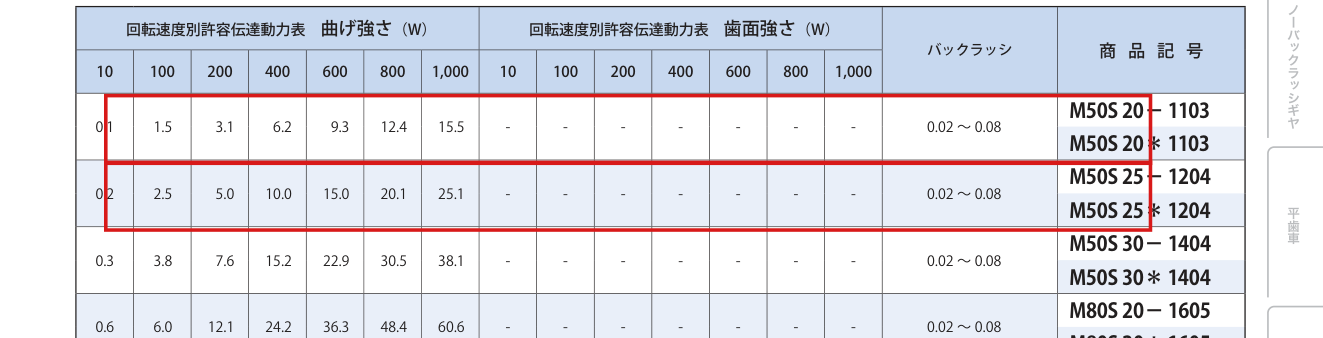
\includegraphics[width=\linewidth]{kg_datasheet_potencia.png}
  \caption{Datasheet KG: potencia admisible a flexión (W) y a picado («--») por velocidad. M50S20: 1,5~W a 100~rpm;
  M50S25: 2,5~W. \emph{Fuente: KG, catálogo KG4001, p.~261.}}
\end{figure}

\begin{table}[H]\centering\small
\begin{tabularx}{\linewidth}{l X X}
\toprule
Condición & Datasheet KG (KG5001, p.~18) & Esta nota\\\midrule
Norma & JGMA 403-01 / 404-01 (alcance: $m\ge1{,}5$) & Shigley cap.~15 (ANSI/AGMA 2003-B97)\\
Modos publicados & Solo flexión & Flexión y picado\\
Ciclos & $\ge10^7$, $K_L=1$ & $2{,}9\times10^7$ (Miner) a 100~rpm\\
Choque & Moderado, $K_O=1{,}25$ & Motor suave, $K_A=1{,}0$\\
Confiabilidad & $K_R=1{,}2$; $C_R=1{,}15$ & $R=0{,}95$: $Y_Z=0{,}895$; $Z_Z=0{,}946$\\
Sentido de carga & Uno solo; con inversión, 2/3 del valor & Ambos sentidos: 70\,\%\\
Lubricación & Baño de aceite 100~cSt & Grasa EP\\
Montaje & Ambos en voladizo & Ambos en voladizo\\
\bottomrule
\end{tabularx}
\end{table}

\paragraph{Validación del cálculo.} El código reproduce el Ejemplo 15-1 de Shigley (mitras de 25 dientes, $P=5$,
$F=1{,}10$~pulg, 180~HB, 600~rpm): da 546 y 460~lbf a flexión y picado, frente a 552,6 y 458,1~lbf del libro.
Las diferencias vienen del redondeo de factores en el ejemplo.

\paragraph{Mismas condiciones.} Se recalculó con Shigley usando las condiciones del datasheet
($K_A=1{,}25$, $Y_Z=1{,}2$, $Z_Z=1{,}15$, $10^7$ ciclos, un sentido):

\begin{table}[H]\centering\small\setlength{\tabcolsep}{5pt}
\begin{tabular}{l r c cc cc}
\toprule
Mitra & rpm & Datasheet KG & \multicolumn{2}{c}{Shigley 170 HB [N\,m]} & \multicolumn{2}{c}{Shigley 200 HB [N\,m]}\\
\cmidrule(lr){4-5}\cmidrule(lr){6-7}
 & & N\,m & Flexión & Picado & Flexión & Picado\\
\midrule
M50S20 & 100  & 0,143 & 0,084 & 0,055 & 0,095 & 0,070\\
       & 1000 & 0,148 & 0,077 & 0,051 & 0,087 & 0,064\\
M50S25 & 100  & 0,239 & 0,135 & 0,108 & 0,153 & 0,137\\
       & 1000 & 0,240 & 0,122 & 0,098 & 0,139 & 0,124\\
\bottomrule
\end{tabular}
\end{table}

\paragraph{¿Dónde puede estar la diferencia?} Shigley da entre 0,51 y 0,58 del datasheet a flexión con los supuestos
de base. Se revisó cada supuesto conservador, acumulando (M50S20, 100~rpm, condiciones KG):

\begin{table}[H]\centering\small\setlength{\tabcolsep}{5pt}
\begin{tabular}{l cc cc}
\toprule
Supuesto & \multicolumn{2}{c}{Flexión} & \multicolumn{2}{c}{Picado}\\
\cmidrule(lr){2-3}\cmidrule(lr){4-5}
 & N\,m & / KG & N\,m & / KG\\
\midrule
Versión anterior: ancho $0{,}3R_e=2{,}12$~mm, 170~HB & 0,071 & 0,50 & 0,047 & 0,33\\
Ancho real 2,5~mm (\textbf{corrección}) & 0,084 & 0,58 & 0,055 & 0,39\\
+ dureza típica 200~HB & 0,095 & 0,66 & 0,070 & 0,49\\
+ $K_R$ de KG leído como $R=0{,}99$ ($Y_Z=1$) & 0,114 & 0,80 & 0,092 & 0,64\\
+ dientes coronados ($Z_{xc}=1{,}5$) & 0,114 & 0,80 & 0,123 & 0,86\\
\bottomrule
\end{tabular}
\end{table}

\begin{itemize}
  \item \textbf{Ancho de diente: error de la versión anterior.} Se había acreditado solo $0{,}3R_e$, pero Shigley usa el ancho
        real: en el Ejemplo 15-1, $F=1{,}10$~pulg supera a $0{,}3A_0=1{,}06$~pulg. Ya está corregido en toda la nota (+18\,\%).
  \item \textbf{Dureza.} 170~HB es el mínimo de la norma del S45C; lo habitual sin tratar es 180--220~HB. Es el supuesto que más
        mueve el picado. \textbf{Se resuelve midiendo la dureza de una mitra.}
  \item \textbf{Confiabilidad.} Se tomó el $K_R=1{,}2$ de KG como el $Y_Z=1{,}2$ de AGMA ($R\approx0{,}998$). Si en JGMA equivale
        a $R\approx0{,}99$, Shigley sube un 20\,\%. No se pudo confirmar sin la norma JGMA.
  \item \textbf{Coronamiento.} Sin dato de KG se supuso diente sin coronar. Si está coronado, el picado sube un tercio.
  \item \textbf{Ninguno de los dos métodos cubre el módulo 0,5.} AGMA se desarrolló para engranajes más grandes y Shigley
        fija $Y_x=0{,}5$ por debajo de $m=1{,}6$; JGMA 403 empieza en $m=1{,}5$. El 20\,\% restante no se puede resolver por cálculo.
  \item \textbf{Conclusión:} el datasheet no está mal. Vale para sus condiciones (un sentido, aceite, $10^7$ ciclos) y no publica
        el picado. Llevado al servicio de la rueda con su propia regla de 2/3 da 0,095\Nm, entre los 0,090 y 0,108\Nm de esta nota.
\end{itemize}

\begin{figure}[H]\centering
  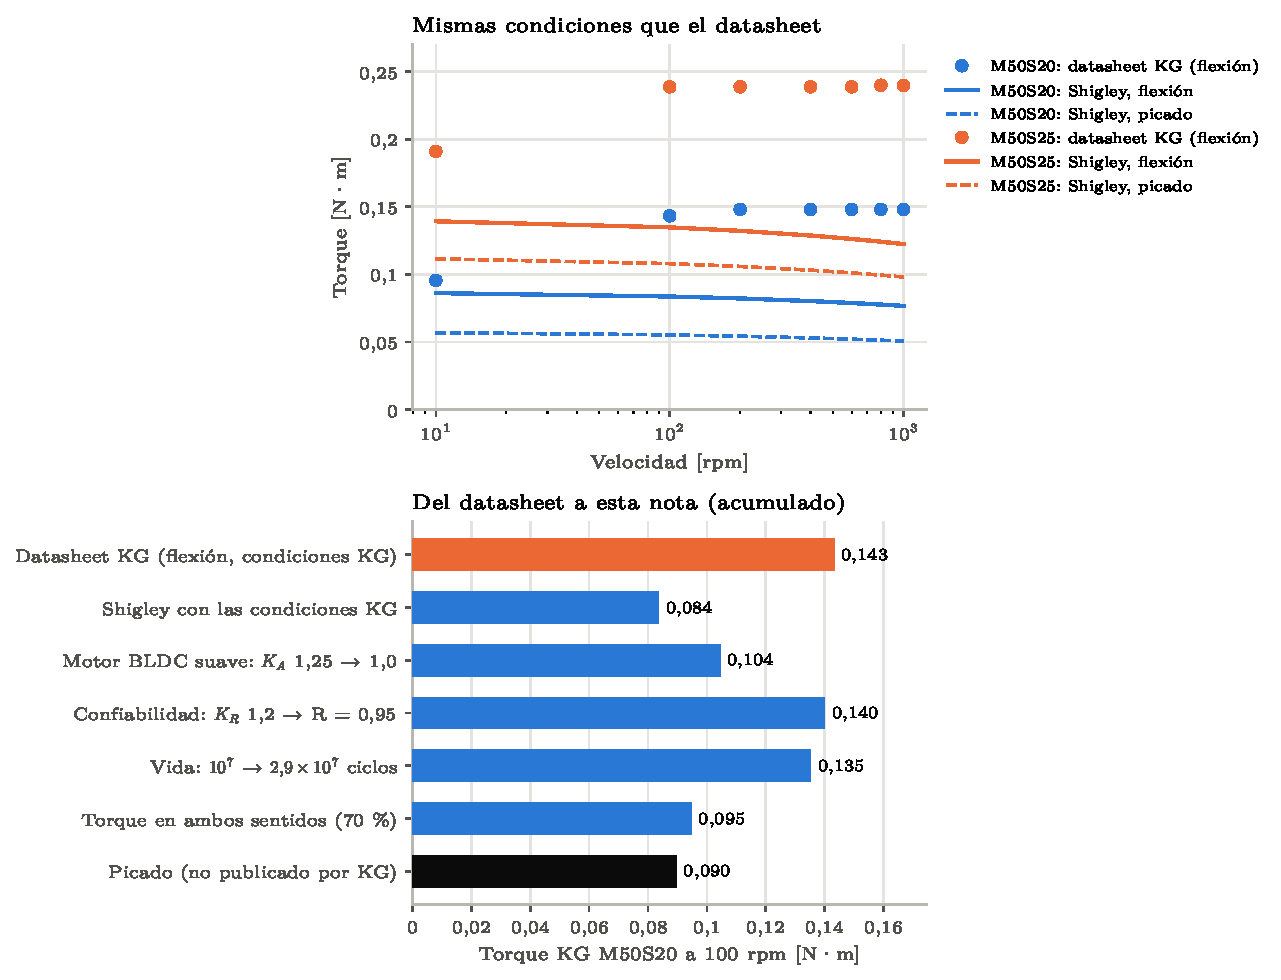
\includegraphics[width=\linewidth]{fig_datasheet.pdf}
  \caption{Arriba: datasheet KG frente a Shigley en las condiciones del datasheet (170~HB). Abajo: del valor del datasheet al
  torque admisible de esta nota, cambiando una condición por vez.}
  \label{fig:datasheet}
\end{figure}

\textbf{Del datasheet a esta nota} (fig.~\ref{fig:datasheet}, abajo): el método baja el valor de 0,143 a 0,084\Nm.
El motor suave ($\times1{,}25$) y la confiabilidad del 95\,\% en lugar de $K_R=1{,}2$ ($\times1{,}34$) lo suben a 0,140.
La vida más larga ($\times0{,}97$) y la carga en ambos sentidos ($\times0{,}70$) lo llevan a 0,095\Nm a flexión,
y el picado fija el admisible en \textbf{0,090\Nm} (170~HB).

%-----------------------------------------------------------------------
\section{Diseños analizados}
Para una mitra 1:1 de 20° Shigley pide al menos 16 dientes (tabla 13-3). Con $d_a=m(z+\sqrt2)\le11{,}5$~mm,
el mayor módulo normalizado posible es 0,6 (z16 o z17): m\,0,7 z16 ya mide 12,2~mm. Las mitras KG M50S25 (13,2~mm),
RS PRO 521-5780 (13,9~mm) y m\,0,6 z21 (13,4~mm) quedan fuera.

\begin{table}[H]\centering\small\setlength{\tabcolsep}{4pt}
\begin{tabular}{l l r r r r r r r}
\toprule
Diseño & Material & $m$ & $z$ & $d_e$ & $d_a$ & $b$ & $Y_J$ & $Z_I$\\
 & & mm & & mm & mm & mm & & \\
\midrule
KG M50S20 & S45C, 170 o 200 HB & 0,5 & 20 & 10,0 & 10,71 & 2,5 & 0,200 & 0,062\\
KG M50B20 & Latón C3604B & 0,5 & 20 & 10,0 & 10,71 & 2,5 & 0,200 & 0,062\\
A medida & SCM440 bonificado 300 HB & 0,5 & 20 & 10,0 & 10,71 & 2,5 & 0,200 & 0,062\\
A medida & SCM415 carb. 58--62 HRC & 0,5 & 20 & 10,0 & 10,71 & 2,5 & 0,200 & 0,062\\
A medida & SCM415 carb. 58--62 HRC & 0,6 & 17 & 10,2 & 11,05 & 2,5 & 0,189 & 0,059\\
\bottomrule
\end{tabular}
\end{table}

\begin{itemize}
  \item \textbf{Geometría} ($\delta=45^\circ$): $d_e=mz$, $R_e=d_e/(2\sin\delta)$, $d_a=d_e+2m\cos\delta$.
        Se acredita el ancho real $b$, como en el Ejemplo 15-1.
  \item $Y_J$ y $Z_I$ salen de las figuras 15-7 y 15-6; para 17 dientes se interpolaron entre 16 y 20.
  \item \textbf{m\,0,5 z20 a medida:} misma geometría que la mitra actual, se reemplaza sin tocar la carcasa.
  \item \textbf{m\,0,6 z17:} ancho de 2,5~mm, con la misma proporción $b/R_e$ que las mitras KG. Gana un 16\,\% sobre la
        m\,0,5 z20 carburizada, pero su distancia de montaje es distinta.
\end{itemize}

%-----------------------------------------------------------------------
\section{Método}\label{sec:metodo}
Shigley, cap.~15, ecuaciones AGMA para cónicos rectos en unidades SI, con $W^t$ la fuerza tangencial en el diámetro exterior.
El torque admisible es el menor entre flexión y picado:
\begin{align}
\sigma_F &= \frac{W^t}{b}\,\frac{K_A K_v}{m_{et}}\,\frac{Y_x K_{H\beta}}{Y_\beta Y_J}
  \;\le\; \sigma_{FP}=\frac{0{,}70\,\sigma_{F\,\lim}\,Y_{NT}}{S_F\,K_\theta\,Y_Z}
  && \text{ec. (15-3), (15-4)}\\
\sigma_H &= Z_E\left(\frac{W^t}{b\,d_e\,Z_I}\,K_A K_v K_{H\beta} Z_x Z_{xc}\right)^{1/2}
  \;\le\; \sigma_{HP}=\frac{\sigma_{H\,\lim}\,Z_{NT}\,Z_W}{S_H\,K_\theta\,Z_Z}
  && \text{ec. (15-1), (15-2)}\\
T_{adm} &= \frac{d_e}{2}\,\min\!\left(W^t_F;\;W^t_H\right)
\end{align}

\begin{table}[H]\centering\small
\begin{tabularx}{\linewidth}{l c X}
\toprule
Factor & Valor & Criterio (Shigley 8.ª ed.)\\\midrule
$K_A$ sobrecarga & 1,00 & BLDC con perfil suave. Con golpes de rueda, 1,25 (fig.~\ref{fig:sens}).\\
$K_v$ dinámico & $\approx1{,}04$ & Ec. (15-5) y (15-6) con $Q_v=6$.\\
$Y_x$, $Z_x$ tamaño & 0,5 & Ec. (15-10) y (15-9): $m_{et}<1{,}6$ mm, $b<12{,}7$ mm.\\
$K_{H\beta}$ distribución & 1,25 & Ec. (15-11), $K_{mb}=1{,}25$: ambos en voladizo.\\
$Z_{xc}$ coronamiento & 2,0 & Ec. (15-12): sin coronamiento garantizado.\\
$Y_\beta$ curvatura & 1 & Ec. (15-13): dientes rectos.\\
$Y_{NT}$, $Z_{NT}$ ciclos & ec. & Ec. (15-15) y (15-14), figs.~15-9 y 15-8.\\
$Y_Z$, $Z_Z$ confiabilidad & 0,895 / 0,946 & Ec. (15-20) con $R=0{,}95$; $Z_Z=\sqrt{Y_Z}$.\\
$K_\theta$, $Z_W$ & 1 & Ec. (15-18) y (15-16): menos de 120\,°C, mismo material.\\
$S_F$, $S_H$ & 1 & Capacidad nominal; el margen lo dan $R$ y los supuestos.\\
\bottomrule
\end{tabularx}
\end{table}

\paragraph{Materiales.}
El S45C sin tratar entra como acero templado total grado~1. Con 170~HB (mínimo de JIS G4051):
$\sigma_{F\,\lim}=0{,}30\,\text{HB}+14{,}48=65{,}5$~MPa y $\sigma_{H\,\lim}=2{,}35\,\text{HB}+162{,}89=562$~MPa, ec.~(15-23) y (15-22);
con 200~HB, 74,5 y 633~MPa.
El SCM440 bonificado a 300~HB, con las mismas ecuaciones, da 104,5 y 868~MPa.
El SCM415 carburizado toma 206,8 y 1379~MPa (30 y 200~kpsi; tablas 15-6 y 15-4, grado~1).
El latón no está en Shigley: se escaló desde el S45C por la relación de límites de fatiga (138/285) a flexión y por la dureza (100/170) a picado.
$Z_E$ sale de la ec.~(15-21): 189,4 para acero-acero y 134,1\,$\sqrt{\text{MPa}}$ para latón-latón.

\paragraph{Ejemplo: KG M50S20, 170 HB, servicio normal a 100 rpm.}
\begin{align*}
N_L &= 2\times(100\cdot60\cdot20\cdot12\cdot10)=2{,}88\times10^{7}
  &&\Rightarrow Y_{NT}=0{,}966,\; Z_{NT}=1{,}238\\
\sigma_{FP} &= 0{,}70\times65{,}5\times0{,}966/0{,}895 = 49{,}5\ \text{MPa}
  &&\Rightarrow T_F=0{,}095\ \text{N\,m}\\
\sigma_{HP} &= 562\times1{,}238/0{,}946 = 736\ \text{MPa}
  &&\Rightarrow T_H=\mathbf{0{,}090}\ \text{N\,m}\ \text{(picado)}
\end{align*}

%-----------------------------------------------------------------------
\section{Comportamiento con la velocidad y sensibilidad}
Con más velocidad hay más ciclos en la vida y el torque admisible baja. Las mitras de acero mejorado quedan limitadas
por flexión; el S45C de 170~HB a 100~rpm queda al límite entre flexión y picado.

\begin{figure}[H]\centering
  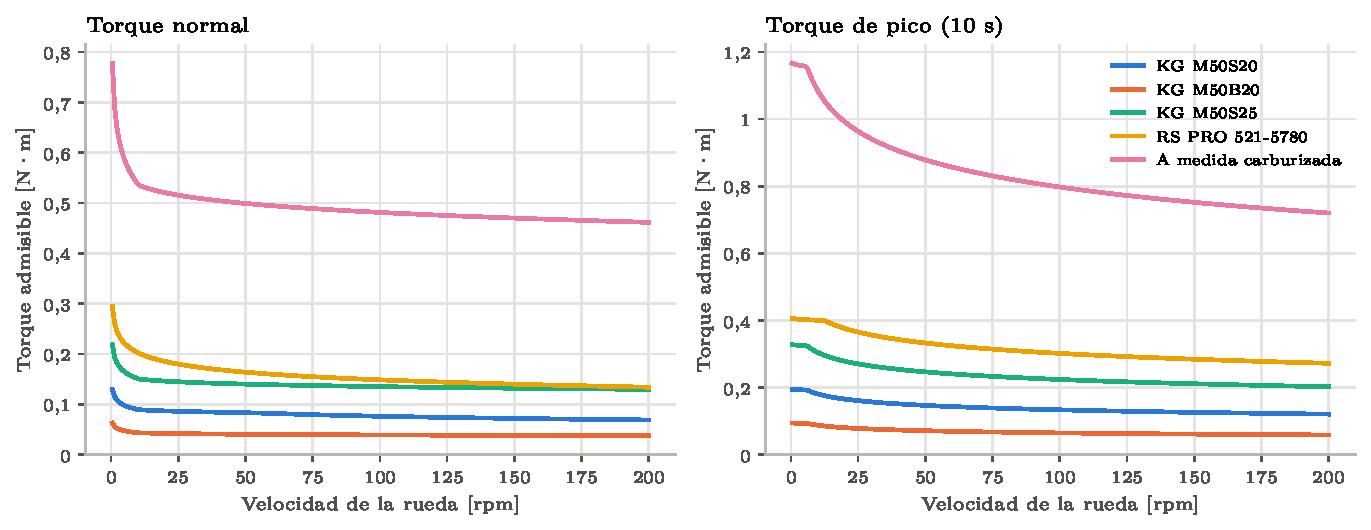
\includegraphics[width=\linewidth]{fig_rpm.pdf}
  \caption{Torque admisible en función de la velocidad de la rueda.}
\end{figure}

\begin{figure}[H]\centering
  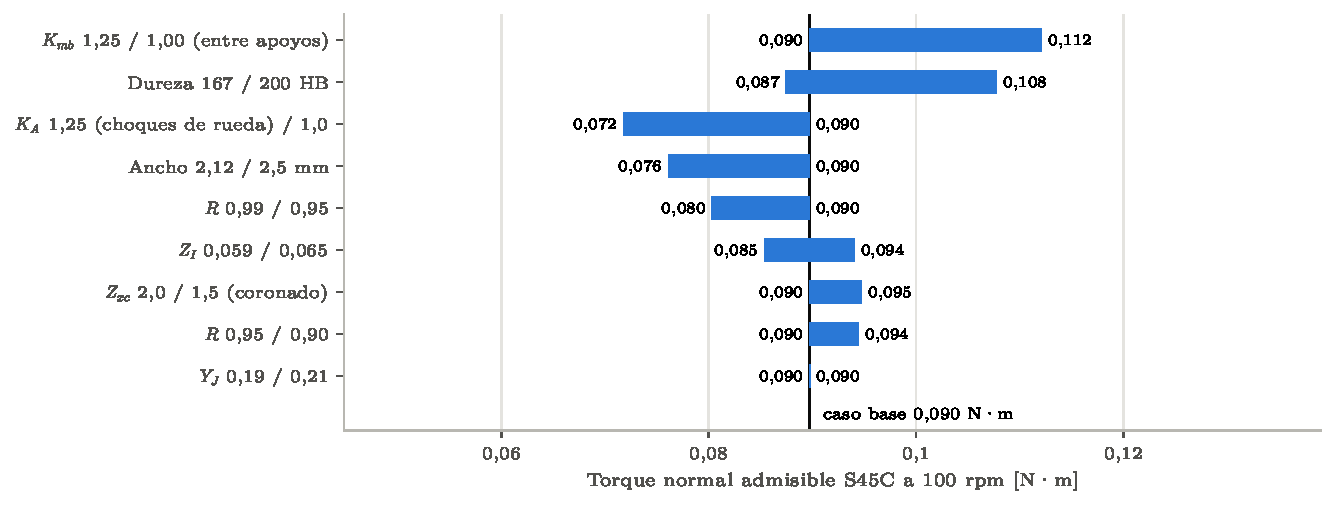
\includegraphics[width=\linewidth]{fig_sensibilidad.pdf}
  \caption{Sensibilidad del torque normal de KG M50S20 (170~HB) a 100~rpm a cada supuesto.}
  \label{fig:sens}
\end{figure}

\begin{figure}[H]\centering
  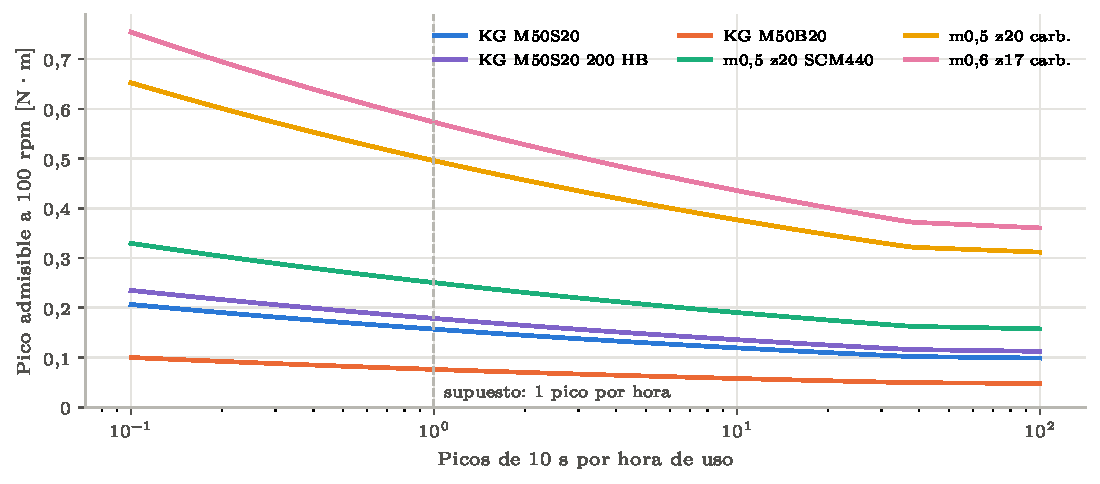
\includegraphics[width=0.72\linewidth]{fig_picos.pdf}
  \caption{Pico admisible a 100~rpm según la frecuencia de picos.}
\end{figure}

Lo que más mueve el resultado es el montaje ($K_{mb}$), la dureza real del S45C y los golpes de rueda ($K_A$).
Si el latón se evalúa con la resistencia a picado del bronce (tabla 14-7), su torque normal baja de 0,046 a 0,023\Nm a 100~rpm.

%-----------------------------------------------------------------------
\section{Falla por flexión del S45C}\label{sec:flexion}
El material elegido es el \textbf{S45C} (mitra KG M50S20). Esta sección separa la falla por flexión (rotura del diente
por fatiga en la raíz) de la de picado, con el uso informado después de la primera versión: \textbf{24~h seguidas una vez
por mes}, en lugar de 20~h, y vidas de 10, 5 y 2~años. El método es el de la sec.~\ref{sec:metodo}; a 100~rpm la vida
es de $3{,}5\times10^7$, $1{,}7\times10^7$ y $6{,}9\times10^6$ ciclos (con Miner, $N_{eval}=2n$).

Se comparan tres escenarios de factores, cada uno acumulando sobre el anterior:
\begin{itemize}
  \item \textbf{Factores de la nota:} los de la tabla de la sec.~\ref{sec:metodo} ($Q_v=6$, $R=0{,}95$, 70\,\% por carga en
        ambos sentidos, ambos engranajes en voladizo, dientes sin coronar).
  \item \textbf{Optimista sin cambiar el montaje:} $Q_v=8$ (casi no influye: $v\approx0{,}05$~m/s), $R=0{,}90$
        ($Y_Z=0{,}85$, el mínimo de la ec.~15-20) y el 100\,\% de la resistencia a flexión. El 70\,\% de Shigley
        (sec.~15-2) corresponde a carga invertida en \emph{cada} ciclo, como en un engranaje loco; en la rueda la inversión
        es ocasional (marcha atrás, frenado).
  \item \textbf{Optimista completo:} además dientes coronados ($Z_{xc}=1{,}5$, ec.~15-12) y un engranaje entre apoyos
        ($K_{mb}=1{,}10$, ec.~15-11). \textbf{Vale solo si el montaje y el tallado lo cumplen}; si no, rige el anterior.
\end{itemize}

\begin{table}[H]\centering\small\setlength{\tabcolsep}{4pt}
\begin{tabular}{l r cc cc}
\toprule
 & & \multicolumn{2}{c}{170 HB [N\,m]} & \multicolumn{2}{c}{200 HB [N\,m]}\\
\cmidrule(lr){3-4}\cmidrule(lr){5-6}
Escenario & Vida & Continuo & Pico 10 s & Continuo & Pico 10 s\\
\midrule
Factores de la nota      & 10 años & 0,094 & 0,154 & 0,107 & 0,175\\
                         &  5 años & 0,096 & 0,167 & 0,110 & 0,190\\
                         &  2 años & 0,099 & 0,186 & 0,113 & 0,212\\
\addlinespace
Optimista sin montaje    & 10 años & 0,144 & 0,235 & 0,164 & 0,267\\
                         &  5 años & 0,147 & 0,255 & 0,167 & 0,290\\
                         &  2 años & 0,152 & 0,284 & 0,172 & 0,323\\
\addlinespace
Optimista completo       & 10 años & 0,164 & 0,267 & 0,186 & 0,303\\
                         &  5 años & 0,167 & 0,290 & 0,190 & 0,330\\
                         &  2 años & 0,172 & 0,323 & 0,196 & 0,368\\
\bottomrule
\end{tabular}
\caption{Torque admisible \emph{a flexión} de la mitra M50S20 (S45C) a 100~rpm, 24~h por mes.}
\label{tab:flexion}
\end{table}

\begin{figure}[H]\centering
  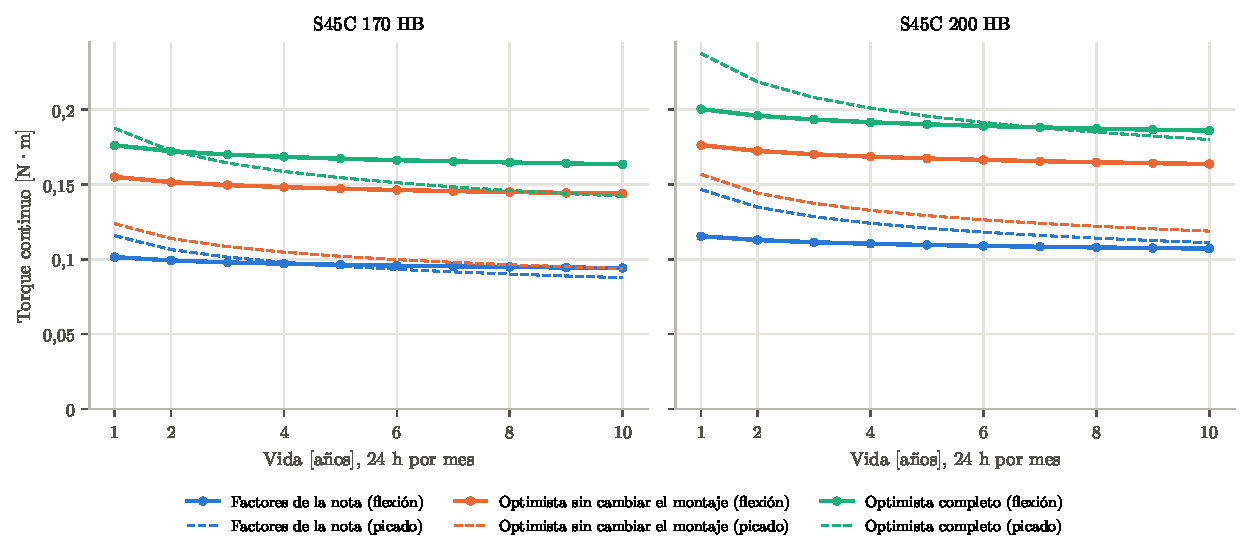
\includegraphics[width=\linewidth]{fig_flexion.pdf}
  \caption{Torque continuo admisible a 100~rpm según la vida: flexión (línea llena) y picado (línea de trazos).
  El admisible de la mitra es el menor de los dos.}
  \label{fig:flexion}
\end{figure}

\begin{itemize}
  \item \textbf{Acortar la vida casi no mueve la flexión:} de 10 a 2~años sube un 5\,\% en continuo y un 20\,\% en picos.
        Entre $10^6$ y $10^8$ ciclos la curva de vida es casi plana ($Y_{NT}\propto N^{-0{,}032}$, ec.~15-15).
  \item \textbf{Lo que más pesa es la carga en ambos sentidos:} pasar del 70\,\% al 100\,\% sube la flexión un 43\,\%.
  \item \textbf{Con los factores de la nota, flexión y picado quedan parejos;} con los optimistas manda el picado,
        salvo en el escenario completo a pocos años, donde los dos se emparejan (fig.~\ref{fig:flexion}). El admisible de la mitra
        es el menor de los dos, no el de la tabla~\ref{tab:flexion}.
\end{itemize}

\paragraph{Rotura estática del diente.} Con la tensión en la raíz igual a la resistencia a la tracción
($S_{ut}\approx3{,}41\,\text{HB}$, ec.~2-17: 580~MPa con 170~HB y 682~MPa con 200~HB), sin factores de vida, confiabilidad
ni seguridad, el diente se rompe de un golpe con \textbf{$\approx$1,2~N\,m (170~HB) y $\approx$1,4~N\,m (200~HB)}
con ambos engranajes en voladizo, y 1,3 a 1,5~N\,m con uno entre apoyos. Es un orden de magnitud, no un valor de diseño:
hay un factor de 6 a 12 frente al admisible a fatiga, que es lo que limita.

\textbf{Limitaciones}
\begin{itemize}
  \item \textbf{Módulo 0,5:} Shigley fija $Y_x=0{,}5$ por debajo de $m=1{,}6$; el método no está validado a este tamaño (sec.~\ref{sec:datasheet}).
  \item \textbf{Picos:} se mantiene 1 pico por hora de uso; con 24~h por mes son 2880, 1440 y 576 picos en 10, 5 y 2~años.
  \item \textbf{Rotura estática:} $S_{ut}$ estimado desde la dureza; el S45C es dúctil y la rotura real suele ser algo mayor.
\end{itemize}

%-----------------------------------------------------------------------
\section{Vida en horas de cada opción}\label{sec:vida}
Esta sección estima \textbf{cuántas horas dura cada opción} con el espectro de carga medido en el robot y con el motor
a pleno, usando \textbf{un único criterio de factores} (tabla~\ref{tab:criterio}): el valor más realista de cada uno, sin acumular supuestos
optimistas ni conservadores. Reemplaza a los escenarios de las secciones anteriores para decidir.

\subsection{Por qué la vida varía tanto con los supuestos}
En el rango de uso las curvas de vida de Shigley son muy planas (ec.~15-15 y 15-14, figs.~15-9 y 15-8):
$Y_{NT}=1{,}6831\,N^{-0{,}0323}$ y $Z_{NT}=3{,}4822\,N^{-0{,}0602}$. Como $\sigma_F\propto T$ y $\sigma_H\propto\sqrt{T}$,
\begin{equation}
N_F\propto T^{-1/0{,}0323}=T^{-31}, \qquad N_H\propto T^{-0{,}5/0{,}0602}=T^{-8{,}3}.
\end{equation}
Un 10\,\% más de torque (o un 10\,\% menos de resistencia) divide la vida por 20 a flexión y por 2,2 a picado.
Por eso, además de las horas, se informa el \textbf{margen de torque}: el torque admisible para 10~años dividido por el
aplicado. El margen cambia poco con los supuestos y es el número que conviene mirar para decidir.

\subsection{Criterio de cálculo}
\begin{table}[!htb]\centering\small
\begin{tabularx}{\linewidth}{l c X}
\toprule
Factor & Valor & Criterio y referencia (Shigley 8.ª ed.)\\\midrule
$K_A$ sobrecarga & 1,0 & Los picos medidos ya están en el espectro; aplicarles $K_A$ los contaría dos veces.\\
$K_v$ dinámico & 1,03 & Ec.~(15-5) y (15-6) con $Q_v=8$ (KG serie M: JIS B1704 grado~3). A 0,05~m/s casi no influye.\\
$Y_x$, $Z_x$ tamaño & 0,5 & Ec.~(15-10) y (15-9): $m<1{,}6$~mm y $b<12{,}7$~mm.\\
$K_{H\beta}$ distribución & 1,25 & Ec.~(15-11) con $K_{mb}=1{,}25$: ambos engranajes en voladizo, lo más probable en un módulo compacto.\\
$Z_{xc}$ coronamiento & 2,0 & Ec.~(15-12): dientes sin coronamiento garantizado.\\
$Y_\beta$ curvatura & 1 & Ec.~(15-13): dientes rectos.\\
$Y_{NT}$, $Z_{NT}$ ciclos & ec. & Ec.~(15-15) y (15-14), figs.~15-9 y 15-8, en su rango de validez $10^2$--$10^{10}$ ciclos.\\
$Y_Z$, $Z_Z$ confiabilidad & 0,850 / 0,922 & Ec.~(15-20) con $R=0{,}90$, el mínimo de su rango: el 90\,\% de los pares supera la vida calculada
                                            (como la vida $L_{10}$ de un rodamiento). $Z_Z=\sqrt{Y_Z}$.\\
$K_\theta$, $Z_W$ & 1 & Ec.~(15-18) y (15-16): menos de 120\,°C; mismo material en los dos engranajes.\\
$S_F$, $S_H$ & 1 & Sin coeficiente adicional: el margen se informa aparte.\\
Carga en ambos sentidos & 100\,\% & Flexión pulsante. El 70\,\% de Shigley (sec.~15-2) es para carga invertida en cada vuelta
                                    (engranaje loco); en la rueda la inversión es ocasional.\\
\bottomrule
\end{tabularx}
\caption{Factores del criterio central (Shigley, cap.~15, unidades SI).}\label{tab:criterio}
\end{table}

\paragraph{Materiales.}
\begin{itemize}
  \item \textbf{S45C de KG:} el catálogo de la serie M recta de S45C indica \emph{sin tratamiento térmico} y no especifica
        dureza~[4]. Se calcula con 200~HB (típico de barra laminada o trefilada) y con 170~HB (cota baja);
        $\sigma_{F\,\lim}$ y $\sigma_{H\,\lim}$ por ec.~(15-23) y (15-22), grado~1. \textbf{Hay que medirla} (sec.~\ref{sec:dureza}).
  \item \textbf{S45C nitrocarburado} (Tenifer/QPQ o gaseoso, $\approx$570\,°C): Shigley no lo tabula. Se supone
        $+30$\,\% en $\sigma_{H\,\lim}$ y $+20$\,\% en $\sigma_{F\,\lim}$ sobre el mismo acero sin tratar, por la diferencia entre
        las categorías de material de ISO~6336-5~[5]. \textbf{Supuesto a validar en banco.}
  \item \textbf{Latón C3604B:} escalado desde el S45C como en la sec.~\ref{sec:metodo}; Shigley no lo cubre.
  \item \textbf{SCM415 carburizado:} 206,8 y 1379~MPa (30 y 200~kpsi), tablas~15-6 y 15-4, grado~1.
  \item \textbf{SCM440 bonificado 300~HB:} ec.~(15-23) y (15-22), grado~1.
\end{itemize}

\paragraph{Espectros de carga} (torque por engranaje, 100~rpm, 24~h seguidas por mes $=$ 288~h por año):
\begin{itemize}
  \item \textbf{Uso real medido:} torque oscilante entre 0,05 y 0,20\Nm, tomado como senoide (60 niveles de igual duración),
        más picos de 0,30\Nm.
  \item \textbf{Motor a pleno:} 0,40\Nm continuo (máximo continuo del motor) más picos de 0,50\Nm (máximo del motor).
  \item \textbf{Picos:} 10~s cada uno, 1 por hora de uso (\textbf{supuesto}); cada pico carga cada diente
        $100\cdot10/60=16{,}7$ veces. A 100~rpm cada diente suma 6000 ciclos por hora; en 10~años, $1{,}73\times10^7$
        ciclos continuos y $4{,}8\times10^4$ en picos.
\end{itemize}

\paragraph{Vida.} Para cada nivel de torque $T_i$ se despeja $N_i$, los ciclos hasta la falla, igualando la tensión de
trabajo con la admisible: $\sigma_F(T_i)=\sigma_{FP}(N_i)$ y $\sigma_H(T_i)=\sigma_{HP}(N_i)$ (ec.~15-3, 15-4, 15-1 y 15-2).
El daño por hora se suma con la regla de Miner (Shigley, sec.~6-15):
\begin{equation}
D_h=\sum_i \frac{n_i}{N_i}, \qquad \text{vida}=\frac{1}{D_h}\ \text{horas},
\end{equation}
por separado para flexión y para picado; manda el que llega antes a $D=1$. Si un nivel de torque no supera la
resistencia a $10^{10}$ ciclos no suma daño. Si supera la resistencia aun a $10^2$ ciclos (flexión) o $10^3$ (picado),
la opción se informa como \textbf{no admisible}: está fuera de las curvas de Shigley y fallaría tempranamente, sin
que se pueda cuantificar cuándo. Por encima de $10^5$~h ($>$340 años) se informa \textbf{no limita}.

\paragraph{Ejemplo: KG M50S20, 200~HB, sin tratar, 0,20\Nm constante.}
\begin{align*}
W^t &= 2T/d_e = 2\cdot0{,}20/0{,}010 = 40{,}0\ \text{N}\\
\sigma_F &= \frac{W^t}{b}\,\frac{K_A K_v}{m_{et}}\,\frac{Y_x K_{H\beta}}{Y_\beta Y_J}\\
  &= \frac{40{,}0}{2{,}5}\cdot\frac{1{,}0\cdot1{,}029}{0{,}5}\cdot\frac{0{,}5\cdot1{,}25}{1\cdot0{,}200} = 102{,}9\ \text{MPa}\\
Y_{NT} &= \frac{\sigma_F\,Y_Z}{\sigma_{F\,\lim}} = \frac{102{,}9\cdot0{,}850}{74{,}5}=1{,}174
  \;\Rightarrow\; N_F=\left(\frac{1{,}174}{6{,}1514}\right)^{-1/0{,}1192}=1{,}1\times10^{6}\ \text{ciclos}\ (181\ \text{h})\\
\sigma_H &= Z_E\left(\frac{W^t}{b\,d_e\,Z_I}\,K_A K_v K_{H\beta} Z_x Z_{xc}\right)^{1/2}\\
  &= 189{,}4\left(\frac{40{,}0}{2{,}5\cdot10\cdot0{,}062}\cdot1{,}029\cdot1{,}25\cdot0{,}5\cdot2{,}0\right)^{1/2} = 1091\ \text{MPa}\\
Z_{NT} &= \frac{\sigma_H\,Z_Z}{\sigma_{H\,\lim}} = \frac{1091\cdot0{,}922}{633}=1{,}589
  \;\Rightarrow\; N_H=\left(\frac{1{,}589}{3{,}4822}\right)^{-1/0{,}0602}=4{,}6\times10^{5}\ \text{ciclos}\ (\mathbf{76\ h})
\end{align*}
($Y_{NT}=1{,}174$ cae en el tramo de $10^3$ a $3\times10^6$ ciclos de la ec.~15-15, $Y_{NT}=6{,}1514\,N^{-0{,}1192}$.) Manda el picado. Con el espectro real el torque pasa la mayor parte del tiempo por debajo de 0,20\Nm y la vida sube a 249~h.

\subsection{Opción 1: mitras KG de stock, con o sin tratamiento}
\begin{table}[H]\centering\small\setlength{\tabcolsep}{3pt}
\resizebox{\linewidth}{!}{\begin{tabular}{l lcc lcc}
\toprule
 & \multicolumn{3}{c}{Uso real (0,05--0,20; picos 0,30)} & \multicolumn{3}{c}{Motor a pleno (0,40; picos 0,50)}\\
\cmidrule(lr){2-4}\cmidrule(lr){5-7}
Opción & Vida & Manda & Margen & Vida & Manda & Margen\\
\midrule
\csname @@input\endcsname tabla_vida_kg.tex 
\bottomrule
\end{tabular}}
\caption{Vida estimada de las mitras KG (d$_a$ 10,71~mm). Margen: torque admisible para 10~años sobre el aplicado,
continuo / pico. «a»: años de uso a 288~h por año.}
\label{tab:vida_kg}
\end{table}

\begin{itemize}
  \item \textbf{Sin tratar no sirve:} con 170~HB los picos de 0,30\Nm superan su resistencia a picado aun para $10^3$ ciclos;
        con 200~HB dura $\approx$250~h ($<$1~año).
  \item \textbf{Nitrocarburada sirve solo para el uso real, y al límite} (margen $\approx$1): $\approx$1100~h (3,7~años) con
        170~HB y $\approx$7400~h (26~años) con 200~HB. La diferencia de dureza cambia la vida 7 veces: \textbf{medirla
        decide la opción}. El tratamiento traslada el límite del picado a la flexión del pie del diente, que depende del núcleo.
  \item \textbf{Con el motor a pleno ninguna mitra KG sirve} (margen 0,3--0,5).
  \item \textbf{El latón no es admisible} en ninguno de los dos casos.
  \item Para usar la KG nitrocarburada hay que \textbf{limitar el driver} a $\approx$0,20\Nm continuo y $\approx$0,30\Nm de pico en
        la mitra, y validarla en banco.
\end{itemize}

\subsection{Opción 2: par a medida con $d_a\le12$~mm}
Mitras 1:1 a 90° de 20°, con $z\ge16$ (Shigley, tabla~13-3) y $d_a=m\,(z+\sqrt2)\le12$~mm.
El ancho se toma $b=0{,}3\,R_e$, la proporción recomendada (Ejemplo~15-1); la fila «como KG» usa el ancho real de la
M50S20 (2,5~mm $=0{,}354\,R_e$), que es el reemplazo directo. $Y_J$ y $Z_I$ salen de las figs.~15-7 y 15-6, interpoladas
entre 16 y 20 dientes.

\begin{table}[H]\centering\small\setlength{\tabcolsep}{2.6pt}
\resizebox{\linewidth}{!}{\begin{tabular}{l cc lcc lcc}
\toprule
 & & & \multicolumn{3}{c}{Uso real} & \multicolumn{3}{c}{Motor a pleno}\\
\cmidrule(lr){4-6}\cmidrule(lr){7-9}
Opción & $d_a$ & $b$ & Vida & Manda & Margen & Vida & Manda & Margen\\
\midrule
\csname @@input\endcsname tabla_vida_12.tex 
\bottomrule
\end{tabular}}
\caption{Vida estimada de los pares a medida. $d_a$ y $b$ en mm.}
\label{tab:vida_12}
\end{table}

\begin{itemize}
  \item \textbf{Todas las carburizadas cubren el uso real} con margen 2 a 3.
  \item \textbf{Para el motor a pleno el óptimo es m\,0,6 z18 carburizada:} $d_a=11{,}65$~mm, módulo normalizado, margen
        1,33 en continuo y 1,84 en picos; no limita en ningún caso. Cambia la distancia de montaje respecto de la KG.
  \item \textbf{Reemplazo directo:} la m\,0,5 z20 carburizada con la geometría de KG (ancho 2,5~mm) da margen 1,16 con el
        motor a pleno ($\approx$98\,000~h). Con $b=0{,}3\,R_e$ cae a 0,99 y $\approx$1700~h: el ancho importa.
  \item \textbf{m\,0,65 z17} rinde más, pero $d_a=11{,}97$~mm no deja margen para la tolerancia del diámetro exterior;
        m\,0,65 es módulo de segunda serie (menos proveedores con herramienta).
  \item \textbf{SCM440 bonificado} alcanza para el uso real (margen 1,25), no para el motor a pleno.
\end{itemize}

\begin{figure}[H]\centering
  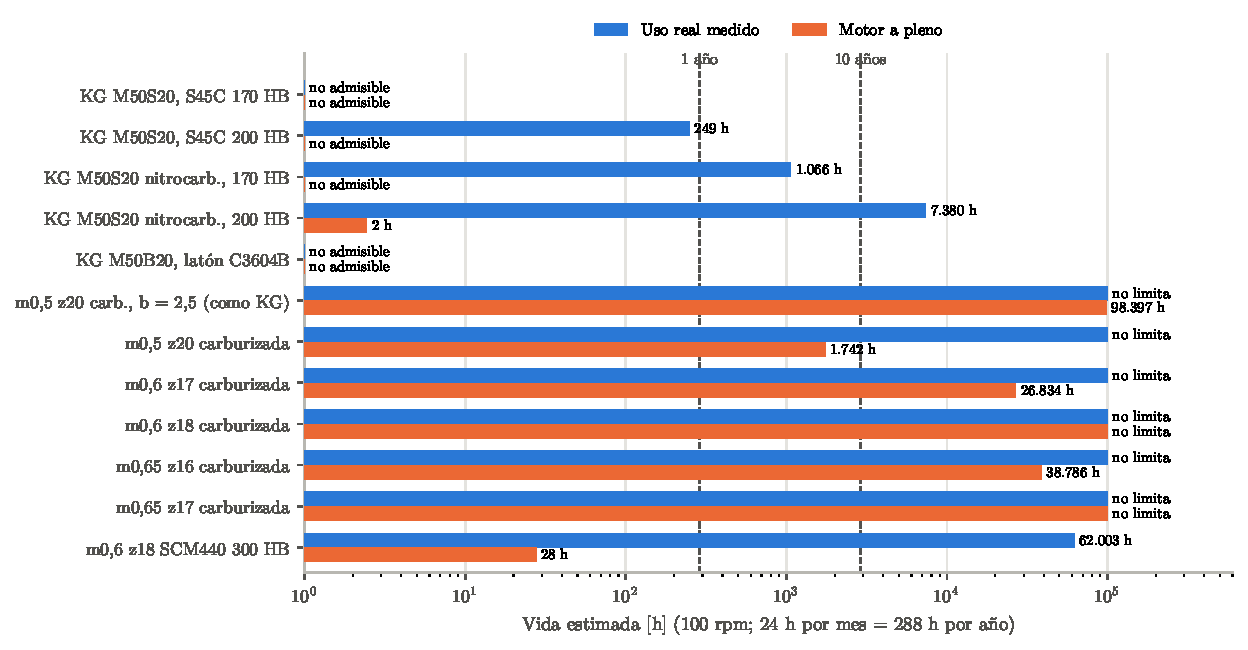
\includegraphics[width=\linewidth]{fig_vida_horas.pdf}
  \caption{Vida estimada de cada opción, uso real y motor a pleno (escala logarítmica).}
  \label{fig:vida_horas}
\end{figure}

\begin{table}[H]\centering\small\setlength{\tabcolsep}{4pt}
\begin{tabular}{l cc cc cc}
\toprule
 & \multicolumn{2}{c}{Resistencia [MPa]} & \multicolumn{2}{c}{Continuo 10 años [N\,m]} & \multicolumn{2}{c}{Picos 10 años [N\,m]}\\
\cmidrule(lr){2-3}\cmidrule(lr){4-5}\cmidrule(lr){6-7}
Opción & $\sigma_{F\,\lim}$ & $\sigma_{H\,\lim}$ & Flexión & Picado & Flexión & Picado\\
\midrule
\csname @@input\endcsname tabla_vida_adm.tex 
\bottomrule
\end{tabular}
\caption{Torque admisible por engranaje para 10~años ($1{,}73\times10^7$ ciclos continuos y $4{,}8\times10^4$ en picos),
criterio central. Es la base de los márgenes de las tablas~\ref{tab:vida_kg} y \ref{tab:vida_12}.}
\end{table}

\subsection{Qué mueve el resultado}
\begin{table}[H]\centering\small
\begin{tabularx}{\linewidth}{l l X}
\toprule
Supuesto & Cambio & Efecto sobre el torque admisible\\\midrule
Dureza del S45C & 170 → 200~HB & $+14$\,\% flexión, $+26$\,\% picado (ec.~15-23 y 15-22). Vida de la KG nitrocarburada: ×7.\\
Inversión de sentido & ocasional → en cada vuelta & $-30$\,\% flexión (sec.~15-2).\\
Montaje & voladizo → uno entre apoyos & $+14$\,\% en ambos modos (ec.~15-11, $K_{mb}=1{,}10$).\\
Coronamiento & sin → con & $+33$\,\% picado (ec.~15-12, $Z_{xc}=1{,}5$).\\
Confiabilidad & 0,90 → 0,99 & $-15$\,\% en ambos modos (ec.~15-20; en picado $T\propto1/Z_Z^2=1/Y_Z$).\\
Frecuencia de picos & 1 → 10 por hora & Vida de la KG nitrocarburada (200~HB, uso real): de 7400 a 970~h ($\div7{,}6$).\\
\bottomrule
\end{tabularx}
\end{table}

\paragraph{Medición de la dureza.}\label{sec:dureza}
Con un durómetro Leeb no es confiable: la mitra pesa 2,6~g y el cubo deja una corona de 2,5~mm, menos que el apoyo del
sensor y muy por debajo de la masa mínima. Se recomienda \textbf{Vickers HV10 en laboratorio}, sobre una mitra cortada y
montada en resina (núcleo del cubo), en 2 o 3 mitras de compras distintas. Si se nitrocarbura, medir en el mismo corte la
microdureza de la capa (HV\,0,1) y su espesor.

\textbf{Limitaciones}
\begin{itemize}
  \item \textbf{Módulo 0,5:} el método no está validado a este tamaño; queda un 20\,\% sin explicar frente al datasheet de KG
        (sec.~\ref{sec:datasheet}).
  \item \textbf{Nitrocarburado:} los incrementos de resistencia son un supuesto; la vida de esa opción debe confirmarse en banco.
  \item \textbf{Espectro:} la senoide y la frecuencia de picos son supuestos; con el registro de torque contra tiempo se
        reemplazan por el espectro medido.
  \item \textbf{Desgaste:} a 0,05~m/s puede limitar antes que el picado y Shigley no lo calcula; depende de la grasa.
  \item \textbf{Eje, prisioneros y rodamientos} no están incluidos: con 0,4--0,5\Nm deben verificarse aparte.
\end{itemize}

%-----------------------------------------------------------------------
\section{Vida con incertidumbre de parámetros}\label{sec:mc}
La sec.~\ref{sec:vida} usa un valor por parámetro. Acá cada parámetro incierto se reemplaza por una distribución y la vida
se calcula para 20\,000 combinaciones al azar (Monte Carlo, semilla fija). El resultado es la \textbf{probabilidad} de que
el par dure una cantidad de horas, por picado o por fatiga a flexión, y qué parámetros explican la dispersión.

\subsection{Datos confirmados}
\begin{table}[H]\centering\small
\begin{tabularx}{\linewidth}{l X}
\toprule
Dato & Valor\\\midrule
Montaje & Ambos engranajes en voladizo: $K_{mb}=1{,}25$ fijo (ec.~15-11).\\
Velocidad & $\approx$100~rpm casi siempre: 6000 ciclos por hora por diente.\\
Sentido de giro & Ida y vuelta frecuente, con tramos de varias vueltas en cada sentido.\\
Picos de torque & Más de 20 por hora con el uso real.\\
Dureza del S45C (KG M50S20) & \textbf{Medida:} 550~HLD con durómetro Leeb, varias lecturas parecidas; el patrón de
                               55,2~HRC da 788~HL. Equivale a $\approx$240~HB.\\
Vida objetivo & 2~años de uso a 24~h por mes $=$ 576~h.\\
\bottomrule
\end{tabularx}
\end{table}

\subsection{Distribuciones de los parámetros}
Cada parámetro incierto, su distribución y su justificación están en la tabla~\ref{tab:distrib}.
\begin{table}[!htb]\centering\footnotesize\setlength{\tabcolsep}{4pt}
\begin{tabularx}{\linewidth}{>{\raggedright\arraybackslash}p{2.9cm} >{\raggedright\arraybackslash}p{4.6cm} X}
\toprule
Parámetro & Distribución & Justificación\\\midrule
Dureza del S45C & Normal 240 $\pm$ 10~HB (1$\sigma$) & Conversión HLD → HB y variación entre lotes de barra.
   Entra en $\sigma_{F\,\lim}$ y $\sigma_{H\,\lim}$ por ec.~(15-23) y (15-22).\\
Resistencia a fatiga del lote & Lognormal: mediana $\sigma_{F\,\lim}/0{,}70$ y $\sigma_{\ln}=0{,}153$ (flexión);
   mediana $\sigma_{H\,\lim}/0{,}837$ y $\sigma_{\ln}=0{,}077$ (picado) & Dispersión implícita en el factor de confiabilidad
   (ec.~15-20, AGMA): $Y_Z=0{,}70$ a $R=0{,}50$, 0,85 a 0,90 y 1,00 a 0,99. En picado $Z_Z=\sqrt{Y_Z}$. Reemplaza a $Y_Z$.\\
Método a m\,0,5 & Lognormal, mediana 1, $\sigma_{\ln}=0{,}10$, independiente en flexión y picado & AGMA no está validado
   a este módulo; queda un 20\,\% sin explicar frente al datasheet de KG (sec.~\ref{sec:datasheet}).\\
Inversión de sentido (flexión) & Uniforme 0,70--1,00 & Shigley sec.~15-2: 0,70 para carga invertida en cada ciclo;
   1,00 para carga pulsante. La ida y vuelta frecuente queda entre ambos.\\
Ciclos por flanco & Uniforme 50--100\,\% del total & Cada flanco trabaja solo en un sentido de giro.\\
Coronamiento $Z_{xc}$ & Uniforme 1,5--2,0 (KG); 1,5--1,75 (a medida) & Ec.~(15-12). KG no lo informa; en la pieza a
   medida se especifica, con tolerancia de fabricación.\\
Nitrocarburado & Triangular (1,10; 1,30; 1,50) en $\sigma_{H\,\lim}$ y (1,00; 1,20; 1,35) en $\sigma_{F\,\lim}$ &
   No está en Shigley; categorías de ISO~6336-5~[5]. Supuesto a validar.\\
Torque máximo continuo & Triangular (0,18; 0,20; 0,23)~N\,m & Medido: oscila entre 0,05 y 0,20~N\,m.\\
Torque de pico & Triangular (0,27; 0,30; 0,35)~N\,m & Medido: picos de $\approx$0,30~N\,m.\\
Picos por hora & Uniforme 20--60 & Informado: más de 20 por hora.\\
Duración de cada pico & Log-uniforme 1--10~s & \textbf{Supuesto}: no está medida.\\
\bottomrule
\end{tabularx}
\caption{Parámetros inciertos del Monte Carlo. Los fijos son los de la tabla~\ref{tab:criterio}
($K_A=1$, $Q_v=8$, $K_{mb}=1{,}25$, $S_F=S_H=1$) y la geometría de cada opción.}\label{tab:distrib}
\end{table}

\paragraph{Modelo.} Es el de la sec.~\ref{sec:vida}: tensiones por ec.~(15-1) y (15-3), curvas de vida por ec.~(15-14) y
(15-15) invertidas en forma exacta por tramos, y daño acumulado por Miner (sec.~6-15) sobre 40 niveles del torque
oscilante más los picos. La resistencia de cada muestra es
\begin{equation}
\sigma_{FP}=\frac{\sigma_{F\,\lim}\,Y_{NT}}{0{,}70}\,e^{-0{,}153\,z_F}\,m_F\,k_{rev},\qquad
\sigma_{HP}=\frac{\sigma_{H\,\lim}\,Z_{NT}}{0{,}837}\,e^{-0{,}077\,z_H}\,m_H,
\end{equation}
con $z\sim N(0,1)$, $m$ el factor del método y $k_{rev}$ el de inversión. \textbf{Control:} con los valores centrales y
$z=1{,}2816$ ($R=0{,}90$) el Monte Carlo da 245~h contra 249~h de la sec.~\ref{sec:vida}; la diferencia viene de usar
40 niveles en lugar de 60.

\subsection{Resultados}
\begin{table}[H]\centering\small\setlength{\tabcolsep}{4pt}
\resizebox{\linewidth}{!}{\begin{tabular}{l l rrr ccc}
\toprule
 & & \multicolumn{3}{c}{Vida [h]} & \multicolumn{2}{c}{Probabilidad de superar} & \\
\cmidrule(lr){3-5}\cmidrule(lr){6-7}
Opción & Carga & P10 & P50 & P90 & 2 años (576 h) & 10 años (2880 h) & Falla por picado\\
\midrule
\csname @@input\endcsname tabla_mc.tex
\bottomrule
\end{tabular}}
\caption{Vida con incertidumbre (20\,000 muestras, 100~rpm, 288~h por año). P10: el 90\,\% de los pares supera esa vida
(equivale a la $L_{10}$ de un rodamiento). P50: mediana. «Falla por picado»: fracción de muestras en que el picado llega
antes que la fatiga a flexión; el resto falla por flexión.}
\label{tab:mc}
\end{table}

\begin{figure}[H]\centering
  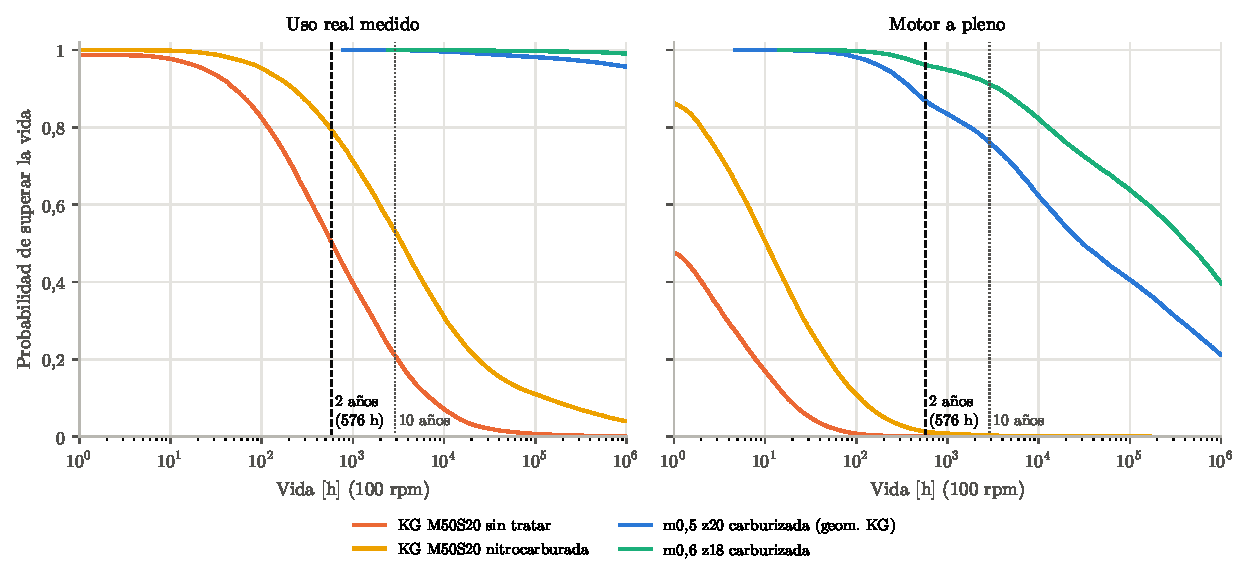
\includegraphics[width=\linewidth]{fig_mc_vida.pdf}
  \caption{Probabilidad de que el par supere una vida dada. Línea de trazos: objetivo de 2~años (576~h).}
  \label{fig:mc}
\end{figure}

\begin{itemize}
  \item \textbf{KG M50S20 sin tratar, uso real:} mediana $\approx$590~h, pero \textbf{solo el 50\,\% llega a 2~años} y el 10\,\%
        falla antes de $\approx$50~h. Con picos frecuentes \textbf{manda la fatiga a flexión} (80\,\% de las muestras), no el picado.
  \item \textbf{KG nitrocarburada, uso real:} el \textbf{79\,\%} llega a 2~años (mediana $\approx$3400~h); P10 $\approx$220~h.
        Mejora mucho, pero no asegura el objetivo: sigue limitada por la flexión del núcleo.
  \item \textbf{Con el motor a pleno ninguna KG sirve} (1\,\% o menos llega a 2~años).
  \item \textbf{m\,0,5 z20 carburizada (geometría KG):} uso real, 100\,\% llega a 2 y a 10~años. Motor a pleno, 87\,\% llega a
        2~años (P10 $\approx$400~h).
  \item \textbf{m\,0,6 z18 carburizada:} uso real, 100\,\%. Motor a pleno, \textbf{96\,\%} llega a 2~años y 91\,\% a 10~años.
\end{itemize}

\subsection{Qué parámetros explican la dispersión}
\begin{table}[H]\centering\small\setlength{\tabcolsep}{4pt}
\begin{tabular}{l cccc}
\toprule
Parámetro & KG sin tratar & KG nitrocarb. & m\,0,5 z20 carb. & m\,0,6 z18 carb.\\
\midrule
\csname @@input\endcsname tabla_mc_sens.tex
\bottomrule
\end{tabular}
\caption{Correlación de rangos (Spearman) entre cada parámetro y la vida, uso real. Positivo: al subir el parámetro
la vida sube. «--»: no aplica a esa opción.}
\end{table}

\begin{itemize}
  \item \textbf{La dispersión propia del material} (resistencia a fatiga del lote) es lo que más pesa y no se puede
        reducir midiendo: es la razón de dar la vida como probabilidad.
  \item \textbf{Lo que sí se puede reducir:} el efecto real de la inversión de sentido sobre la flexión y el factor del método
        a m\,0,5 se cierran con un \textbf{ensayo de banco}; la \textbf{duración de los picos} se cierra con el
        \textbf{registro de torque contra tiempo}.
  \item \textbf{La dureza pesa poco} una vez medida ($\pm$10~HB). El torque máximo continuo casi no pesa: el daño lo hacen los picos.
\end{itemize}

\textbf{Limitaciones}
\begin{itemize}
  \item \textbf{Distribuciones supuestas:} la dispersión de resistencia sale del factor de confiabilidad de AGMA, no de
        ensayos de estas mitras; la duración de los picos no está medida.
  \item \textbf{Extrapolación:} vidas mayores que $10^5$~h ($>$340~años) se informan como tales; superan el rango validado de
        las curvas de vida y solo indican que ese modo no limita.
  \item \textbf{Desgaste, eje, prisioneros y rodamientos} no están incluidos.
\end{itemize}

%-----------------------------------------------------------------------
\section{Fijación al eje y lubricación}
\begin{table}[H]\centering\small\setlength{\tabcolsep}{4pt}
\begin{tabular}{l r r l r r}
\toprule
Diseño & Pico 0 rpm & 2 prisioneros M2,5 & Fijación & \multicolumn{2}{c}{$\tau$ eje [MPa]}\\
\cmidrule(lr){5-6}
 & N\,m & N\,m & & eje 3~mm & eje 4~mm\\
\midrule
KG M50S20 & 0,229--0,261 & 0,28 & prisioneros & 43--49 & --\\
m\,0,5 z20 SCM440 & 0,366 & 0,28 & plano en D / pasador & 69 & 29\\
m\,0,5 z20 carburizada & 0,724 & 0,28 & pasador, eje de 4~mm & 137 & 58\\
m\,0,6 z17 carburizada & 0,838 & 0,28 & pasador, eje de 4~mm & 158 & 67\\
\bottomrule
\end{tabular}
\end{table}
Prisioneros según la tabla 7-4 (n.º 2 $\approx$ M2,5: 85~lbf), con factor de seguridad 2; $\tau=16T/(\pi d^3)$.
Con más capacidad en los dientes, la unión al eje pasa a ser el límite. Un pasador de 1,5~mm a doble corte en eje de 4~mm
(con 200~MPa admisibles) transmite unos 1,4\Nm. El cubo de la m\,0,5 z20 admite agujero de 4~mm (diámetro de fondo $\approx9$~mm).
Hay que revisar también rodamientos y carcasa para los torques de pico.

\textbf{Lubricación.} A 0,03--0,07~m/s no se forma película elastohidrodinámica y el desgaste, que AGMA no calcula, es el modo
de falla a largo plazo. Usar grasa semifluida NLGI 00--0 de complejo de litio con aditivos EP, compartimiento cerrado contra polvo,
reengrase en cada mantenimiento y control del juego después de las primeras campañas. En seco los valores de esta nota no son válidos.

%-----------------------------------------------------------------------
\section{Próximos pasos}
\begin{enumerate}[leftmargin=1.4em]
  \item \textbf{Medir la dureza} de 2 o 3 mitras M50S20 con Vickers HV10 en laboratorio (no con Leeb, sec.~\ref{sec:vida}). Decide si la KG nitrocarburada es viable.
  \item \textbf{Consultar a KG} si los dientes están coronados y qué capacidad a picado dan para $m=0{,}5$.
  \item \textbf{Ensayo de banco} para cerrar el 20\,\% que ningún método resuelve: par M50S20 con grasa EP a 0,10\Nm en ambos
        sentidos, inspeccionando flancos y juego a intervalos fijos de ciclos.
\end{enumerate}

%-----------------------------------------------------------------------
\section{Referencias}
\begin{enumerate}[label={[\arabic*]}, leftmargin=2em]
  \item Budynas, R.\,G. y Nisbett, J.\,K. \emph{Diseño en ingeniería mecánica de Shigley}, 8.ª ed. McGraw-Hill, 2008.
        Cap.~15 (ec. 15-1 a 15-23, tablas 15-4 y 15-6, figs. 15-6 a 15-13, Ejemplo 15-1), tablas 13-3, 7-4 y 14-7.
  \item KG (Kyoiku Gear). Catálogo KG4001, mitras, pp.~233--276 (tabla de potencia, p.~261).
  \item KG. Material de referencia KG5001, p.~18 (condiciones de cálculo) y p.~20 (conversión de potencia).
  \item KG. Catálogo de mitras, ed.~2025, serie M recta de S45C (m\,0,5 a 4): JIS B1704 grado~3, sin tratamiento
        térmico, dureza no especificada. \texttt{kggear.co.jp}, sección de mitras.
  \item ISO 6336-5:2016. \emph{Calculation of load capacity of spur and helical gears --- Part 5: Strength and quality
        of materials}. Categorías de material, entre ellas aceros nitrocarburados.
\end{enumerate}

Cálculo reproducible: \texttt{02489-00-MC001/calculo.py}. Genera las figuras, \texttt{resultados.json} y \texttt{comparacion\_kg.json}.

\end{document}
